\documentclass{beamer}
\usetheme{Antibes}

\usepackage[makeroom]{cancel}

\title[DeepComp]{\textbf{Deep Compositing} \tiny{Using Lie Algebras}}
\author{Minliang LIN\\SIGGRAPH 2017\\Paper Author: Tom Duff}
\date{\tiny\today}

% control sequence whose name is non-letter
% doesn't require either spaces or braces aftet it
\def\*#1{\mathbf{#1}}
\def\Ov{\ \*{\scriptstyle{Over}}\ }
\newcommand{\norm}[1]{\left\lVert#1\right\rVert}

\begin{document}
\frame{\titlepage}

% \begin{frame}
%   \frametitle{Outline}
%   \tableofcontents
% \end{frame}

\section{Background}

\frame{{Author Info}
\begin{itemize}
  \item Tom Duff
  \item Classic papaer of \textit{\textbf{Compositing} Digital Images}, 1984
  \item Fully develop the concept of \textbf{Alpha Compositing} and \textbf{Alpha Channel}
\end{itemize}
\begin{columns}
  \column[]{0.3\textwidth}
  \centering
  
\includegraphics[width=\textwidth]{img/alp}
  \column[]{0.4\textwidth}
  \centering
  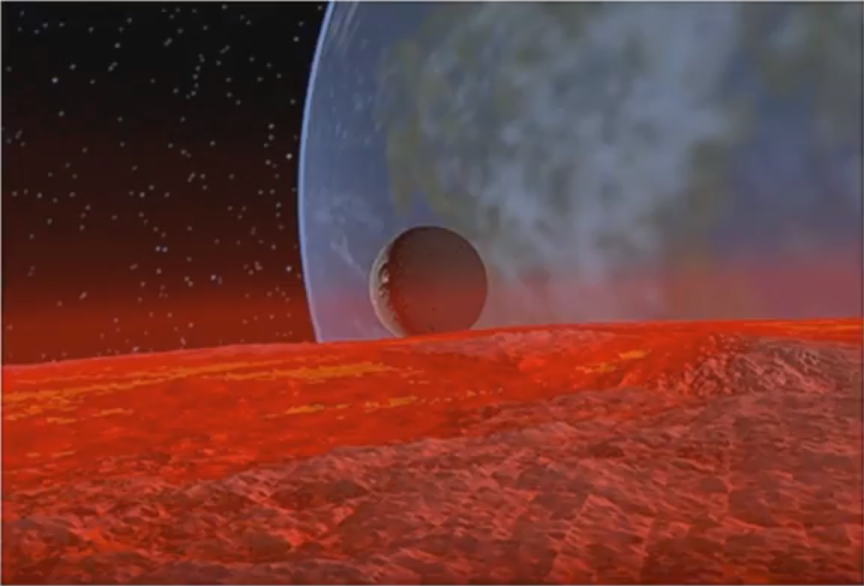
\includegraphics[width=\textwidth]{img/alc2}
  \column[]{0.28\textwidth}
  \centering
  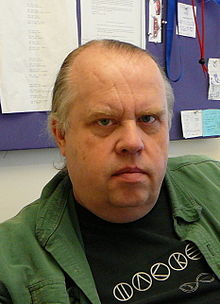
\includegraphics[width=0.7\textwidth]{img/tom}
\end{columns}
}

\frame{{Motivation}
  \begin{itemize}
    \item Nowadays, industrial film scene is a \textbf{compositing} of many parts.
    \begin{itemize}
      \item Dividing and conquer
      \item Reusing
    \end{itemize}
  \end{itemize}
  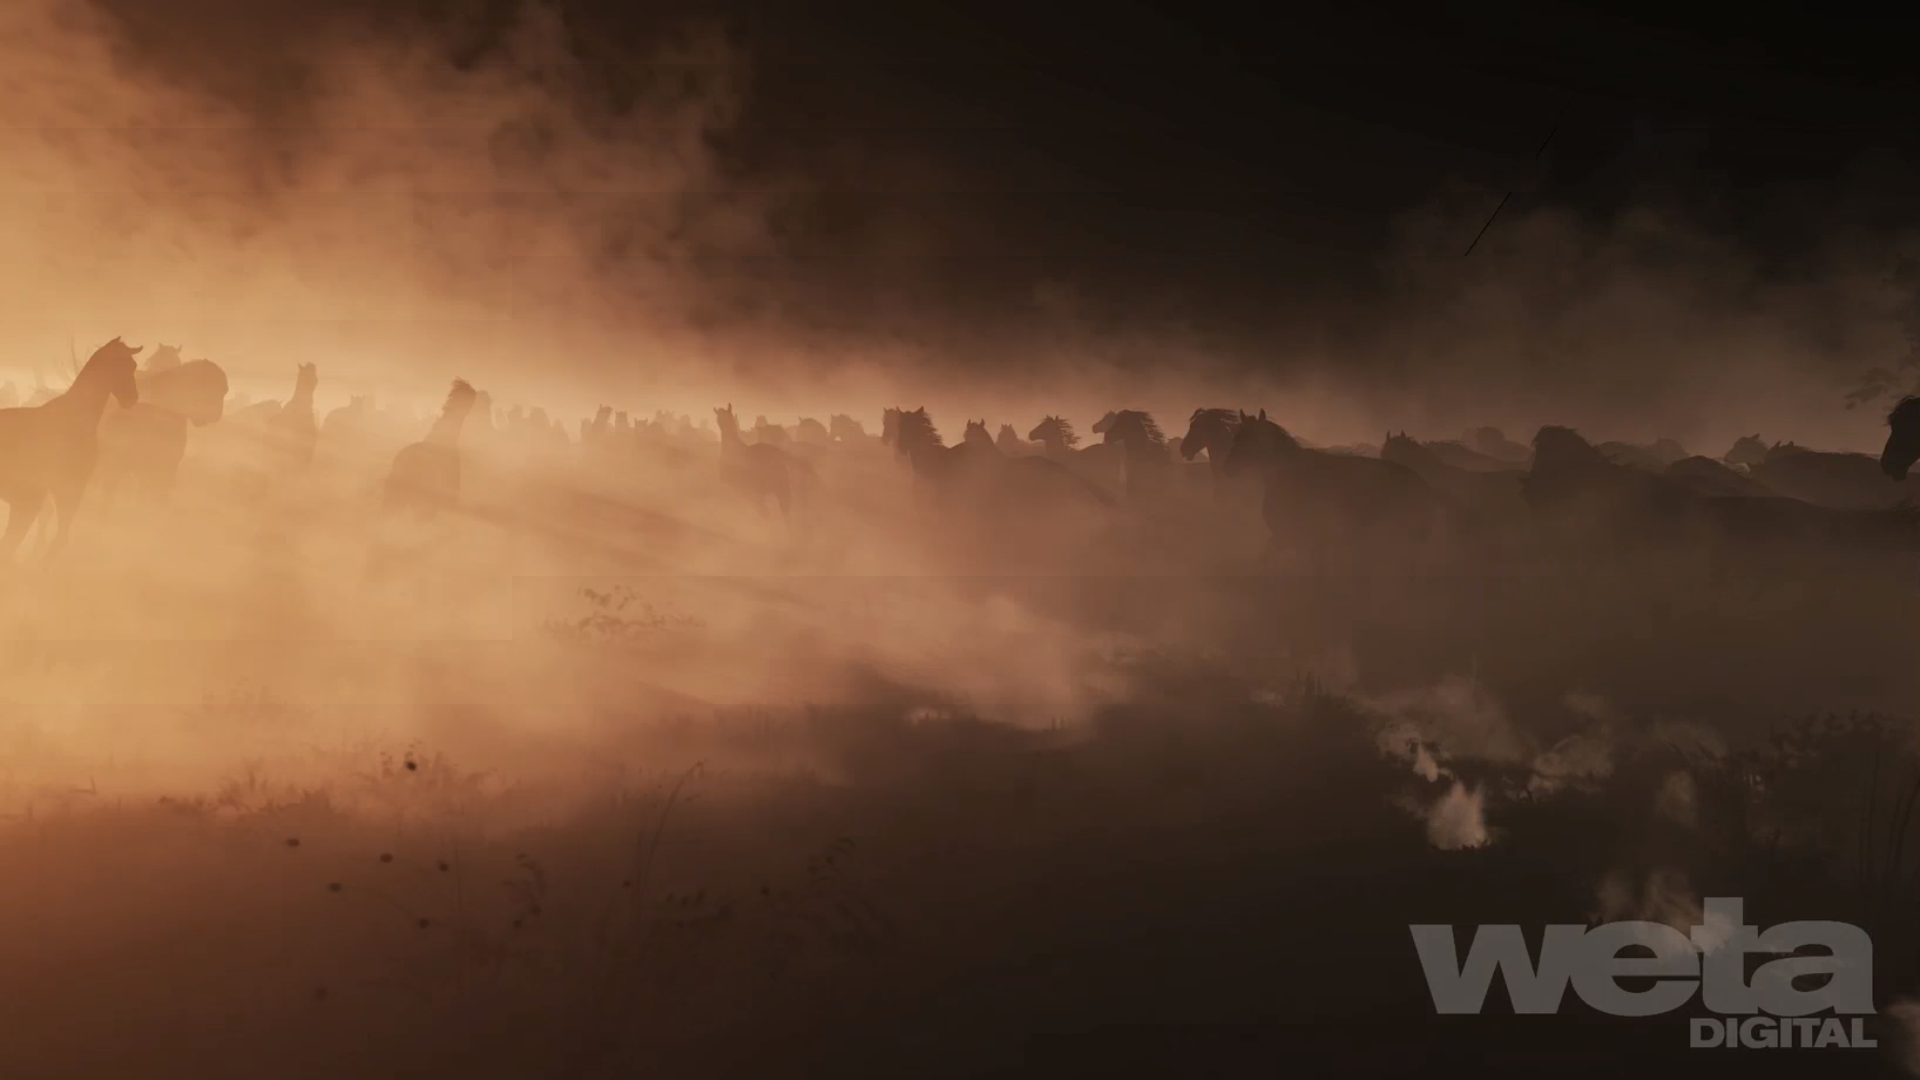
\includegraphics[width=0.8\textwidth]{img/d4}
}

\frame{{Deep Compositing}
\begin{itemize}
  \item Considering special objects, e.g. cloud, fog or shadow
  \item Storing different color for different depth, i.e. \textbf{Volumetric Image}
  \only<2>{
  \item Very useful in industry
  \begin{itemize}
    \item Three awards from \textit{Oscars SciTech}, 2014
    %\item A part that \textit{cannot be turned off} in industrial pipeline
    \item Used in OpenEXR file format
  \end{itemize}
  }
\end{itemize}
\includegraphics<1>[width=0.3\textwidth]{img/c}
\includegraphics<3>[width=\textwidth]{img/cb}
}

\section{Main Idea}

\frame{{Alpha Compositing Review}
\begin{columns}
\column[]{0.7\textwidth}
\begin{itemize}
  \item Pixel Value: $A = (a, \alpha), B = (b, \beta)$
  \begin{itemize}
    \item $a = (R, G, B)$
    \item $\alpha = 0$ for transparent
    \item $\alpha = 1$ for opaque
  \end{itemize}
  \item Compositing: $A\Ov B = A + (1-\alpha)B$
  \item<2> Object color premultiplied by alpha
  \item<2> $a = \alpha a_{origin}, b = \beta b_{origin}$
  \item<2> Not confused with \xcancel{$c = \alpha a + (1-\alpha)\beta b$}.
\end{itemize}
\column[]{0.2\textwidth}

\includegraphics[width=\textwidth]{img/alp}\\
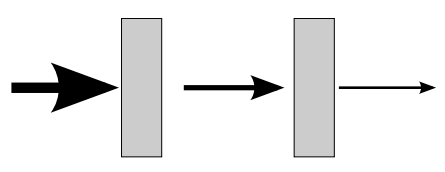
\includegraphics[width=\textwidth]{img/li}
\end{columns}
}

\frame{{Representing Volumetric Image}
\begin{itemize}
  \item Voxelization is expensive.
  \item Interval representation
  \item Assume piecewise constant pixel value in interval
\end{itemize}
\centering

\includegraphics[width=0.8\textwidth]{img/lcode}
}

\frame{{Split And Merge}
\begin{itemize}
  \item \textbf{Assume} constant optical density
  \item Split to length $\lambda, 1-\lambda, \mu, 1-\mu$ (relative length)\\
  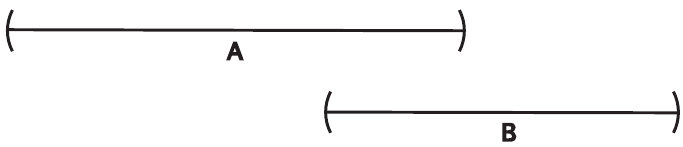
\includegraphics[width=0.4\textwidth]{img/s1}\\
  \item Reassign pixel value $A^\lambda, A^{1-\lambda}, B^{\mu}, B^{1-\mu}$
  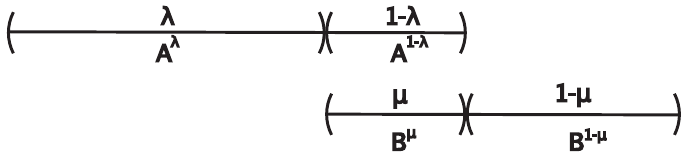
\includegraphics[width=0.6\textwidth]{img/s2}\\
  \item Merge pixel value on common interval $A^{1-\lambda}\otimes B^{\mu}$
  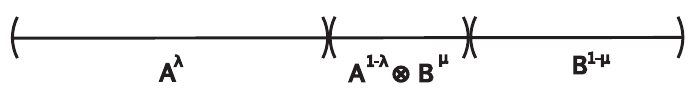
\includegraphics[width=0.6\textwidth]{img/s3}
  \item Finally, $A^\lambda \Ov (( A^{1-\lambda}\otimes B^{\mu}) \Ov B^{1-\mu})$
\end{itemize}
}

\frame{{Split Function}
\begin{itemize}
  \item \textbf{Assume} constant optical density
  \item In other words, interval consists of $n$ tranparent unit
  \item $A^n = \underbrace{A\Ov(A\Ov\cdots\Ov A)\cdots)}_{\text{n times}}=(\sum\limits^{n-1}_{i=0}(1-\alpha)^i)A=\begin{cases}\frac{1-(1-\alpha)^n}{\alpha}A,\ \text{if}\ \alpha\neq 0\\nA,\ \text{if}\ \alpha = 0\end{cases}$
  \item easily generalized to $A^\lambda$
\end{itemize}
\hspace*{5em}
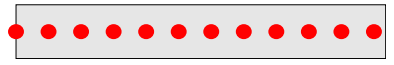
\includegraphics[width=0.3\textwidth]{img/seq}\\
\centering
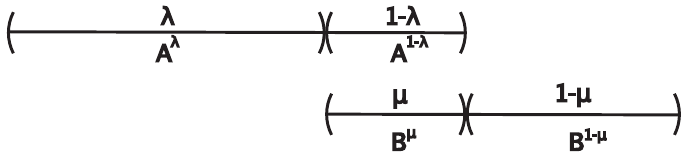
\includegraphics[width=0.6\textwidth]{img/s2}
}

\frame{{Merging Function}
\begin{itemize}
  \item \textbf{Assume} A, B unit occupy the common interval alternately.
  \item $A\otimes B=\lim\limits_{n\to\infty}\underbrace{(A^{1/n}\Ov B^{1/n}\Ov \dots A^{1/n}\Ov B^{1/n})}_{\text{n times}} = \lim\limits_{n\to\infty}(A^{1/n}\Ov B^{1/n})^n$
  \item SymPy: $A\otimes B=\frac{1-(1-\alpha)(1-\beta)}{\log(1-\alpha)+\log(1-\beta)}(\frac{\log(1-\alpha)}{\alpha}A+\frac{\log(1-\beta)}{\beta}B)$
\end{itemize}
\centering
\hspace*{2.5em}
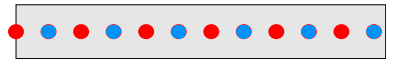
\includegraphics[width=0.16\textwidth]{img/seq2}\\
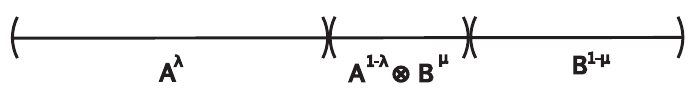
\includegraphics[width=0.8\textwidth]{img/s3}
}

\section{Lie algebras formulation}

\frame{{So Far...}
\begin{itemize}
  \item All formulas are known 6 years ago for industry.
  \item $A^\lambda = \frac{1-(1-\alpha)^n}{\alpha}A,\ \text{if}\ \alpha\neq 0...$
  \item $A\otimes B=\frac{1-(1-\alpha)(1-\beta)}{\log(1-\alpha)+\log(1-\beta)}(\frac{\log(1-\alpha)}{\alpha}A+\frac{\log(1-\beta)}{\beta}B)$
  \item<2> Using monochrome channel $A=(a,\alpha), a=(R)$ for convenience
\end{itemize}
\centering
\includegraphics<2>[width=0.6\textwidth]{img/eq}
}

\frame{{Correspondence}
\begin{itemize}
  \item $A \Ov B$ is hard to analyze, not commute
  \item Over operator cannot give a vector space
  \item $A \otimes B = exp(log A + log B)$
  \item $A^\lambda = exp(\lambda log A)$
  \item $log A, log B$ are in a \textbf{vector space} with addition and scalar multiplication, easy to analyze.
\end{itemize}
}

\section{Application}

\frame{{Interpolation}
\begin{itemize}
  \item $interpolation(A, B, t) = exp((1-t)log A + t log B)$
  \item $interpolation(A^n, B^n, t) = interpolation(A, B, t)^n$
  \item Split invariant
\end{itemize}
\centering
\includegraphics<2>[width=0.6\textwidth]{img/int}
}

\frame{{Compression}
\centering
Compare OpenEXR and new approach.

\includegraphics[width=0.5\textwidth]{img/lcode}\\
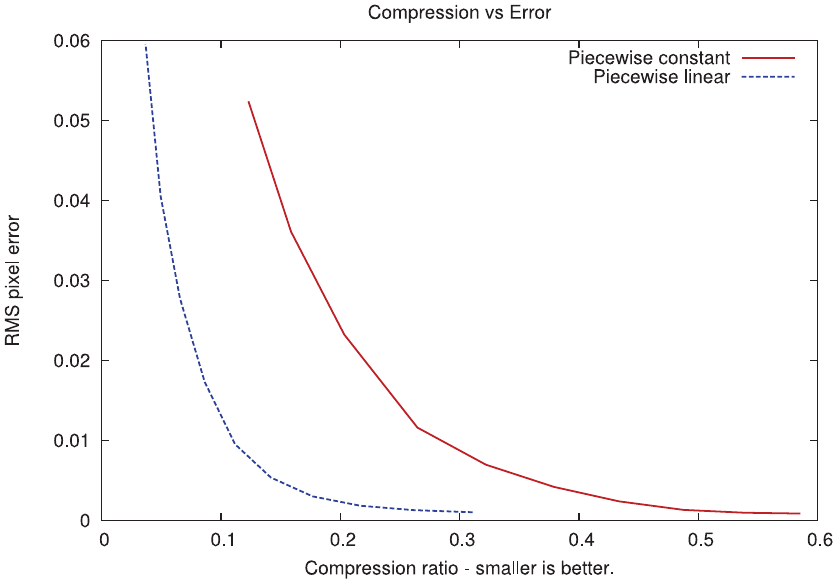
\includegraphics[width=0.7\textwidth]{img/rms}
}

\section{End}
\frame{
\centering\Large Thanks!
}

\end{document}
